\documentclass[border=5pt]{standalone}
\usepackage{tikz}
\usepackage{pgfplots}
\pgfplotsset{compat=1.18}
\usepackage{amsmath,amssymb,amsfonts,bm}
\usepackage{xcolor}

% BRAND colors
\definecolor{tiger}{HTML}{FF5A00}
\definecolor{fire}{HTML}{FF4D00}
\definecolor{flicker}{HTML}{DC4B07}
\definecolor{steel}{HTML}{878F92}
\definecolor{gunmetal}{HTML}{122128}
\definecolor{panel}{HTML}{202E35}

% FIGURE colors
\definecolor{dark_navy}{HTML}{122128}
\definecolor{forgis_orange}{HTML}{FF5A00}
\definecolor{forgis_fire}{HTML}{FF4D00}
\definecolor{forgis_flicker}{HTML}{DC4B07}
\definecolor{blue}{HTML}{3A7BD5}
\definecolor{green}{HTML}{2ECC71}
\definecolor{panelbg}{HTML}{F0F4F8}
\definecolor{warm_amber}{HTML}{FFF3CD}

% LEVEL colors
\definecolor{L1bg}{HTML}{E0F2F1}
\definecolor{L1border}{HTML}{00796B}
\definecolor{L2bg}{HTML}{FFF8E1}
\definecolor{L2border}{HTML}{F57F17}
\definecolor{L3bg}{HTML}{F3E5F5}
\definecolor{L3border}{HTML}{6A1B9A}
\definecolor{L4bg}{HTML}{FFEBEE}
\definecolor{L4border}{HTML}{B71C1C}

\usetikzlibrary{arrows.meta, positioning, calc, fit, shapes.geometric, 
  decorations.pathreplacing, backgrounds, patterns, shadows}

\begin{document}
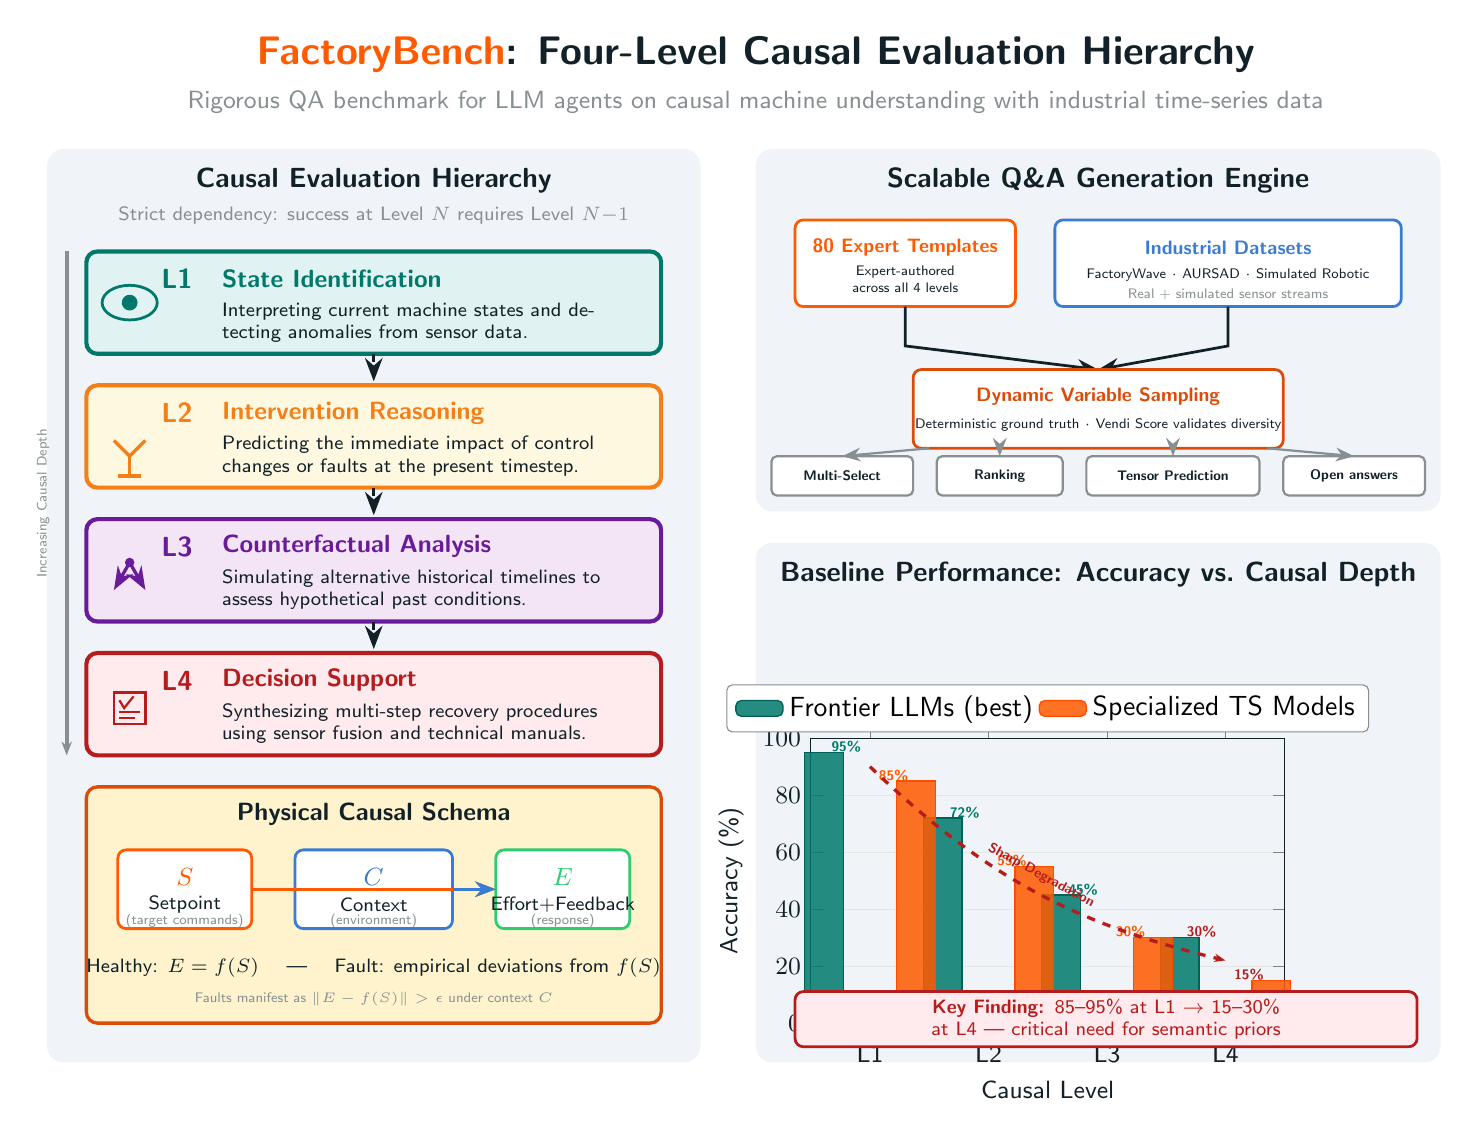
\begin{tikzpicture}[
  every node/.style={font=\sffamily},
  >=Stealth
]

% ====== TITLE ======
\node[font=\sffamily\bfseries\Large, text=gunmetal] at (8.5, 16.8) 
  {\textcolor{forgis_orange}{FactoryBench}: Four-Level Causal Evaluation Hierarchy};
\node[font=\sffamily\small, text=steel] at (8.5, 16.2) 
  {Rigorous QA benchmark for LLM agents on causal machine understanding with industrial time-series data};

% ====== LEFT COLUMN: HIERARCHY ======
% Background panel
\begin{scope}
\fill[panelbg, rounded corners=6pt] (-0.5, 4.0) rectangle (7.8, 15.6);
\node[font=\sffamily\bfseries\normalsize, text=gunmetal] at (3.65, 15.2) 
  {Causal Evaluation Hierarchy};
\node[font=\sffamily\scriptsize, text=steel] at (3.65, 14.75) 
  {Strict dependency: success at Level $N$ requires Level $N{-}1$};

% --- L1 ---
\fill[L1bg, rounded corners=4pt] (0.0, 13.0) rectangle (7.3, 14.3);
\draw[L1border, line width=1.5pt, rounded corners=4pt] (0.0, 13.0) rectangle (7.3, 14.3);
\node[font=\sffamily\bfseries, text=L1border] at (1.15, 13.95) {L1};
\node[font=\sffamily\bfseries\small, text=L1border, anchor=west] at (1.6, 13.95) {State Identification};
\node[font=\sffamily\scriptsize, text=gunmetal, text width=5.0cm, anchor=west] at (1.6, 13.4) 
  {Interpreting current machine states and detecting anomalies from sensor data.};
% Icon: eye
\draw[L1border, line width=1pt] (0.55, 13.65) ellipse (0.35 and 0.22);
\fill[L1border] (0.55, 13.65) circle (0.1);

% --- L2 ---
\fill[L2bg, rounded corners=4pt] (0.0, 11.3) rectangle (7.3, 12.6);
\draw[L2border, line width=1.5pt, rounded corners=4pt] (0.0, 11.3) rectangle (7.3, 12.6);
\node[font=\sffamily\bfseries, text=L2border] at (1.15, 12.25) {L2};
\node[font=\sffamily\bfseries\small, text=L2border, anchor=west] at (1.6, 12.25) {Intervention Reasoning};
\node[font=\sffamily\scriptsize, text=gunmetal, text width=5.0cm, anchor=west] at (1.6, 11.7) 
  {Predicting the immediate impact of control changes or faults at the present timestep.};
% Icon: wrench
\draw[L2border, line width=1.2pt] (0.35, 11.9) -- (0.55, 11.7) -- (0.75, 11.9);
\draw[L2border, line width=1.2pt] (0.55, 11.7) -- (0.55, 11.45);
\draw[L2border, line width=1.2pt] (0.4, 11.45) -- (0.7, 11.45);

% --- L3 ---
\fill[L3bg, rounded corners=4pt] (0.0, 9.6) rectangle (7.3, 10.9);
\draw[L3border, line width=1.5pt, rounded corners=4pt] (0.0, 9.6) rectangle (7.3, 10.9);
\node[font=\sffamily\bfseries, text=L3border] at (1.15, 10.55) {L3};
\node[font=\sffamily\bfseries\small, text=L3border, anchor=west] at (1.6, 10.55) {Counterfactual Analysis};
\node[font=\sffamily\scriptsize, text=gunmetal, text width=5.0cm, anchor=west] at (1.6, 10.0) 
  {Simulating alternative historical timelines to assess hypothetical past conditions.};
% Icon: branching arrows
\draw[L3border, line width=1.2pt, ->] (0.55, 10.35) -- (0.35, 10.0);
\draw[L3border, line width=1.2pt, ->] (0.55, 10.35) -- (0.75, 10.0);
\fill[L3border] (0.55, 10.35) circle (0.06);

% --- L4 ---
\fill[L4bg, rounded corners=4pt] (0.0, 7.9) rectangle (7.3, 9.2);
\draw[L4border, line width=1.5pt, rounded corners=4pt] (0.0, 7.9) rectangle (7.3, 9.2);
\node[font=\sffamily\bfseries, text=L4border] at (1.15, 8.85) {L4};
\node[font=\sffamily\bfseries\small, text=L4border, anchor=west] at (1.6, 8.85) {Decision Support};
\node[font=\sffamily\scriptsize, text=gunmetal, text width=5.0cm, anchor=west] at (1.6, 8.3) 
  {Synthesizing multi-step recovery procedures using sensor fusion and technical manuals.};
% Icon: checklist
\draw[L4border, line width=1pt] (0.35, 8.7) rectangle (0.75, 8.3);
\draw[L4border, line width=0.8pt] (0.42, 8.6) -- (0.48, 8.5) -- (0.6, 8.65);
\draw[L4border, line width=0.8pt] (0.42, 8.45) -- (0.68, 8.45);
\draw[L4border, line width=0.8pt] (0.42, 8.37) -- (0.62, 8.37);

% --- Dependency arrows ---
\draw[gunmetal, line width=1.2pt, ->, dashed] (3.65, 13.0) -- (3.65, 12.65);
\draw[gunmetal, line width=1.2pt, ->, dashed] (3.65, 11.3) -- (3.65, 10.95);
\draw[gunmetal, line width=1.2pt, ->, dashed] (3.65, 9.6) -- (3.65, 9.25);

% --- Difficulty arrow on the side ---
\draw[steel, line width=1.5pt, -{Stealth[length=5pt]}] (-0.25, 14.3) -- (-0.25, 7.9);
\node[font=\sffamily\tiny, text=steel, rotate=90] at (-0.55, 11.1) {Increasing Causal Depth};

% ====== Physical Causal Schema ======
\fill[warm_amber, rounded corners=4pt] (0.0, 4.5) rectangle (7.3, 7.5);
\draw[flicker, line width=1.2pt, rounded corners=4pt] (0.0, 4.5) rectangle (7.3, 7.5);
\node[font=\sffamily\bfseries\small, text=gunmetal] at (3.65, 7.15) {Physical Causal Schema};

% S node
\fill[white, rounded corners=3pt] (0.4, 5.7) rectangle (2.1, 6.7);
\draw[forgis_orange, line width=1pt, rounded corners=3pt] (0.4, 5.7) rectangle (2.1, 6.7);
\node[font=\sffamily\bfseries\small, text=forgis_orange] at (1.25, 6.35) {$S$};
\node[font=\sffamily\scriptsize, text=gunmetal] at (1.25, 6.0) {Setpoint};
\node[font=\sffamily\tiny, text=steel] at (1.25, 5.8) {(target commands)};

% C node
\fill[white, rounded corners=3pt] (2.65, 5.7) rectangle (4.65, 6.7);
\draw[blue, line width=1pt, rounded corners=3pt] (2.65, 5.7) rectangle (4.65, 6.7);
\node[font=\sffamily\bfseries\small, text=blue] at (3.65, 6.35) {$C$};
\node[font=\sffamily\scriptsize, text=gunmetal] at (3.65, 6.0) {Context};
\node[font=\sffamily\tiny, text=steel] at (3.65, 5.8) {(environment)};

% E node
\fill[white, rounded corners=3pt] (5.2, 5.7) rectangle (6.9, 6.7);
\draw[green, line width=1pt, rounded corners=3pt] (5.2, 5.7) rectangle (6.9, 6.7);
\node[font=\sffamily\bfseries\small, text=green] at (6.05, 6.35) {$E$};
\node[font=\sffamily\scriptsize, text=gunmetal] at (6.05, 6.0) {Effort+Feedback};
\node[font=\sffamily\tiny, text=steel] at (6.05, 5.8) {(response)};

% Arrows S->E, C->E
\draw[forgis_orange, line width=1pt, ->] (2.1, 6.2) -- (5.2, 6.2);
\draw[blue, line width=1pt, ->] (4.65, 6.2) -- (5.2, 6.2);

% Equation
\node[font=\sffamily\scriptsize, text=gunmetal] at (3.65, 5.2) 
  {Healthy: $E = f(S)$ \quad | \quad Fault: empirical deviations from $f(S)$};
\node[font=\sffamily\tiny, text=steel] at (3.65, 4.8) 
  {Faults manifest as $\|E - f(S)\| > \epsilon$ under context $C$};

\end{scope}

% ====== RIGHT COLUMN: GENERATION + RESULTS ======
% --- Q&A Generation Engine ---
\begin{scope}
\fill[panelbg, rounded corners=6pt] (8.5, 11.0) rectangle (17.2, 15.6);
\node[font=\sffamily\bfseries\normalsize, text=gunmetal] at (12.85, 15.2) 
  {Scalable Q\&A Generation Engine};

% Template box
\fill[white, rounded corners=3pt] (9.0, 13.6) rectangle (11.8, 14.7);
\draw[forgis_orange, line width=1pt, rounded corners=3pt] (9.0, 13.6) rectangle (11.8, 14.7);
\node[font=\sffamily\bfseries\scriptsize, text=forgis_orange] at (10.4, 14.35) {80 Expert Templates};
\node[font=\sffamily\tiny, text=gunmetal, text width=2.4cm, align=center] at (10.4, 13.95) 
  {Expert-authored across all 4 levels};

% Datasets box
\fill[white, rounded corners=3pt] (12.3, 13.6) rectangle (16.7, 14.7);
\draw[blue, line width=1pt, rounded corners=3pt] (12.3, 13.6) rectangle (16.7, 14.7);
\node[font=\sffamily\bfseries\scriptsize, text=blue] at (14.5, 14.35) {Industrial Datasets};
\node[font=\sffamily\tiny, text=gunmetal] at (14.5, 14.0) {FactoryWave $\cdot$ AURSAD $\cdot$ Simulated Robotic};
\node[font=\sffamily\tiny, text=steel] at (14.5, 13.75) {Real + simulated sensor streams};

% Arrow down
\draw[gunmetal, line width=1pt, ->] (10.4, 13.6) -- (10.4, 13.1) -- (12.85, 12.8);
\draw[gunmetal, line width=1pt, ->] (14.5, 13.6) -- (14.5, 13.1) -- (12.85, 12.8);

% Dynamic sampling box
\fill[white, rounded corners=3pt] (10.5, 11.8) rectangle (15.2, 12.8);
\draw[flicker, line width=1pt, rounded corners=3pt] (10.5, 11.8) rectangle (15.2, 12.8);
\node[font=\sffamily\bfseries\scriptsize, text=flicker] at (12.85, 12.45) {Dynamic Variable Sampling};
\node[font=\sffamily\tiny, text=gunmetal] at (12.85, 12.1) {Deterministic ground truth $\cdot$ Vendi Score validates diversity};

% Output formats
% Output formats
% 1. Multi-Select
\fill[white, rounded corners=2pt] (8.7, 11.2) rectangle (10.5, 11.7);
\draw[steel, line width=0.8pt, rounded corners=2pt] (8.7, 11.2) rectangle (10.5, 11.7);
\node[font=\sffamily\tiny\bfseries, text=gunmetal] at (9.6, 11.45) {Multi-Select};

% 2. Ranking
\fill[white, rounded corners=2pt] (10.8, 11.2) rectangle (12.4, 11.7);
\draw[steel, line width=0.8pt, rounded corners=2pt] (10.8, 11.2) rectangle (12.4, 11.7);
\node[font=\sffamily\tiny\bfseries, text=gunmetal] at (11.6, 11.45) {Ranking};

% 3. Tensor Prediction
\fill[white, rounded corners=2pt] (12.7, 11.2) rectangle (14.9, 11.7);
\draw[steel, line width=0.8pt, rounded corners=2pt] (12.7, 11.2) rectangle (14.9, 11.7);
\node[font=\sffamily\tiny\bfseries, text=gunmetal] at (13.8, 11.45) {Tensor Prediction};

% 4. Open answers
\fill[white, rounded corners=2pt] (15.2, 11.2) rectangle (17.0, 11.7);
\draw[steel, line width=0.8pt, rounded corners=2pt] (15.2, 11.2) rectangle (17.0, 11.7);
\node[font=\sffamily\tiny\bfseries, text=gunmetal] at (16.1, 11.45) {Open answers};

% Arrows connecting from Dynamic Sampling to outputs
\draw[steel, line width=0.8pt, ->] (10.7, 11.8) -- (9.6, 11.7);
\draw[steel, line width=0.8pt, ->] (11.6, 11.8) -- (11.6, 11.7);
\draw[steel, line width=0.8pt, ->] (13.8, 11.8) -- (13.8, 11.7);
\draw[steel, line width=0.8pt, ->] (15.0, 11.8) -- (16.1, 11.7);

\end{scope}

% ====== PERFORMANCE CHART ======
\begin{scope}
\fill[panelbg, rounded corners=6pt] (8.5, 4.0) rectangle (17.2, 10.6);
\node[font=\sffamily\bfseries\normalsize, text=gunmetal] at (12.85, 10.2) 
  {Baseline Performance: Accuracy vs.\ Causal Depth};

\begin{axis}[
  at={(9.2cm, 4.5cm)},
  width=7.6cm,
  height=5.2cm,
  ymin=0, ymax=100,
  xmin=0.5, xmax=4.5,
  xtick={1,2,3,4},
  xticklabels={L1, L2, L3, L4},
  ylabel={Accuracy (\%)},
  xlabel={Causal Level},
  ylabel style={font=\sffamily\small, text=gunmetal},
  xlabel style={font=\sffamily\small, text=gunmetal},
  tick label style={font=\sffamily\small, text=gunmetal},
  ybar,
  bar width=14pt,
  ymajorgrids=true,
  grid style={gray!20},
  axis line style={gunmetal},
  clip=false,
  every axis plot/.append style={fill opacity=0.85},
  legend style={
    at={(0.5, 1.02)},
    anchor=south,
    legend columns=2,
    font=\sffamily\tiny,
    draw=steel,
    fill=white,
    rounded corners=2pt,
  },
  area legend,
]

% High range bars (best models)
\addplot[
  fill=L1border,
  draw=L1border!80!black,
  line width=0.5pt,
] coordinates {
  (0.8, 95)
  (1.8, 72)
  (2.8, 45)
  (3.8, 30)
};

% Low range bars (weaker models)
\addplot[
  fill=forgis_orange,
  draw=forgis_fire,
  line width=0.5pt,
] coordinates {
  (1.2, 85)
  (2.2, 55)
  (3.2, 30)
  (4.2, 15)
};

\legend{Frontier LLMs (best), Specialized TS Models}

% Annotations
\node[font=\sffamily\tiny\bfseries, text=L1border] at (axis cs:0.8, 97) {95\%};
\node[font=\sffamily\tiny\bfseries, text=forgis_orange] at (axis cs:1.2, 87) {85\%};
\node[font=\sffamily\tiny\bfseries, text=L1border] at (axis cs:1.8, 74) {72\%};
\node[font=\sffamily\tiny\bfseries, text=forgis_orange] at (axis cs:2.2, 57) {55\%};
\node[font=\sffamily\tiny\bfseries, text=L1border] at (axis cs:2.8, 47) {45\%};
\node[font=\sffamily\tiny\bfseries, text=forgis_orange] at (axis cs:3.2, 32) {30\%};
\node[font=\sffamily\tiny\bfseries, text=L4border] at (axis cs:3.8, 32) {30\%};
\node[font=\sffamily\tiny\bfseries, text=L4border] at (axis cs:4.2, 17) {15\%};

% Degradation arrow
\draw[L4border, line width=1.2pt, -{Stealth[length=4pt]}, dashed] 
  (axis cs:1.0, 90) to[bend right=15] node[midway, above, sloped, font=\sffamily\tiny\bfseries, text=L4border] {Sharp Degradation} (axis cs:4.0, 22);

\end{axis}

% Key insight box
\fill[L4bg, rounded corners=3pt] (9.0, 4.2) rectangle (16.9, 4.9);
\draw[L4border, line width=1pt, rounded corners=3pt] (9.0, 4.2) rectangle (16.9, 4.9);
\node[font=\sffamily\scriptsize, text=L4border, text width=7.5cm, align=center] at (12.95, 4.55) 
  {\textbf{Key Finding:} 85--95\% at L1 $\rightarrow$ 15--30\% at L4 — critical need for semantic priors};

\end{scope}

\end{tikzpicture}
\end{document}